% Kopfzeile beim Kapitelanfang:
\fancypagestyle{plain}{
%Kopfzeile links bzw. innen
\fancyhead[L]{\calligra\Large Vorlesung Nr. 15}
%Kopfzeile rechts bzw. außen
\fancyhead[R]{\calligra\Large 02.12.2013}
}
%Kopfzeile links bzw. innen
\fancyhead[L]{\calligra\Large Vorlesung Nr. 15}
%Kopfzeile rechts bzw. außen
\fancyhead[R]{\calligra\Large 02.12.2013}
% **************************************************
%
\setcounter{chapter}{8}
\setcounter{section}{11}
\section*{Graph der Exponentialfunktion}
\begin{tikzpicture}[domain=-3:2, scale=0.85, prefix="plots/", smooth]
    \draw[very thin,color=gray] (-3.1,-0.1) grid (1.6,4.1);
    \draw[->] (-3.2,0) -- (1.7,0) node[right] {$x$};
    \draw[->] (0,-0.1) -- (0,4.2) node[right] {$y$};
    \draw[dashed] (1, 2.7182) -- (1,0) node[below] {$1$};
    \draw[dashed] (1, 2.7182) -- (0,2.7182) node[left] {$e$}; 
    \draw[color=red, domain=-3:1.5] plot[id=v15g1] function{exp(x)} node[right] {};
\end{tikzpicture}

\section*{Berechnung von $e^x$}
$x\in \R \Rarr x = g+x', x' \in [0,1), g \in \Z$\\
$\Rarr e^x = e^g * e^{x'}$\\
Bestimme $e^x$ für $0≤ x≤1$\\
$e^x = \sum_{k=0}^{∞} \frac{x^k}{k!} = \sum_{k=0}^{n} \frac{x^k}{k!} + R_{n+1}(x)$\\
$R_{n+1}(x)= \sum_{k=n+1}^{∞}\frac{x^k}{k!}$ Restglied\\
$|x|≤1 \Rarr |R_{n+1}(x)| ≤ \sum_{k=n+1}^{∞} \frac{|x|^k}{k!} = \frac{|x|^{n+1}}{(n+1)!}\left[ 1 + \frac{|x|}{n+2} + \frac{|x|^2}{(n+2)(n+3)} + ... \right] ≤ \frac{|x|^{n+1}}{(n+1)!} \left[ 1 + \frac{|x|}{2} +\frac{|x|^2}{2\cdot 2} + ... \right] ≤ \frac{|x|^{n+1}}{(n+1)!} \underbrace{\left[ 1 + \frac{1}{2} + \frac{1}{2^2} + \frac{1}{2^3} \right]}_{=2 (\text{geometrische Reihe})}$
\section{Satz: Restgliedabschätzung für exp}
$x\in\C, |x|≤1 \Rarr e^x = \sum_{k=0}^{n} \frac{x^k}{k!} + R_{n+1}(x)$ wobei:\\
$|R_{n+1}|≤2\cdot \underbrace{\frac{|x|^{n+1}}{(n+1)!}}_{\text{Betrag des 1. weggelassenen Gliedes}}$ dabei "<" falls $x\neq 0$\\
\section{Korollar}
$e$ ist irrational.
\subsection*{Beweis}
Angenommen: $e= \frac{m}{n}\in \Q, m,n \in \N$\\
$\Rarr s:= \left(e-\sum_{k=0}^{n} \frac{1}{k!}\right) \cdot n!$\\
Aber: $(*) = R_{n+1}(1) \Rarr s < n! \cdot \frac{2}{(n+1)!} \Rarr s< \frac{2}{n+1} \lightning$
\subsection*{Bemerkung}
e ist nicht nur irrational, sondern auch transzendent. Es gibt also kein Polynom mit rationalen Koeffizienten, sodass p(e)=0.
\section{Bemerkung}
$e^x = \lim\limits_{n\to ∞} \left( 1 + \frac{x}{n} \right)^n$\\
Beweis später.
\section*{Anwendung: Kontinuierliche Verzinsung}
Anfangskapital $K$\\
Zinssatz für 1 Jahr: p\% (Zinsfuß)\\
Verzinsung in jedem $\frac{1}{n}$-ten Jahr $\frac{p}{n}$\% Zinsen auf jeweils das aktuelle Kapital\\
Kapital nach einem Jahr: $K \cdot \left( 1 + \frac{p}{n} \cdot \frac{1}{100} \right)^n \underset{\longrightarrow}{n\to ∞} K \cdot e^{\frac{p}{100}}$
\section*{Sinus und Cosinus}
Vorüberlegung: $z\in \C \Rarr \overline{e^z} = e^{\overline{z}}$\\
Denn: $e^{\overline{z}} = \sum_{k=0}^{∞} \frac{\overline{z}^k}{k!} = \lim\limits_{n\to ∞} \sum_{k=0}^{n} \frac{\overline{z}^k}{k!} = \lim\limits_{n\to ∞} \overline{\sum_{k=0}^{n}\frac{z^k}{k!}} = \overline{\lim\limits_{n\to ∞} \sum_{k=0}^{n}\frac{z^k}{k!}}$
$\overline{e^{ix}} = e^{-ix} \Rarr |e^{ix}| = 1$\\

\begin{wrapfigure}{l}{0.23\textwidth}
\vspace{-20pt}
	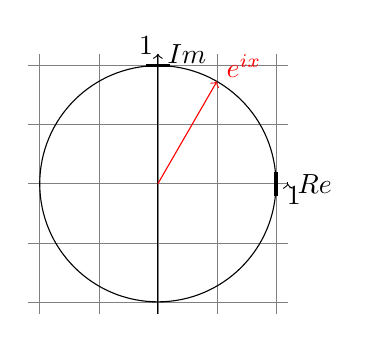
\begin{tikzpicture}[domain=-1.2:1.2, scale=1.5, prefix="plots/", smooth]
	% Raster einzeichnen
    \draw[very thin,color=gray,step=0.5] (-1.1,-1.1) grid (1.1,1.1);
    % Koordinatensystem
    \draw[->] (1.1, 0) -- (1.1,0) node[right] {$Re$}; 
    \draw[->] (0, -1.1) -- (0,1.1) node[right] {$Im$};
    \draw[-, very thick]  (1, 0.1) -- (1, -0.1) node[below, right] {1};
    \draw[-, very thick]  (0.1, 1) -- (-0.1, 1) node[left, above] {1};
    % Einheitskreis zeichnen
    \draw[color=black] (0,0) circle (1);
    % Pfeil einzeichnen
	\draw[<-,color=red] (60:1)++(0,0) -- (0,0);
	\draw[color=red] (0.5,1) node[right] {$e^{ix}$};
	\end{tikzpicture}
\vspace{-50pt}
\end{wrapfigure}

\section{Definition: Sinus / Cosinus auf $\R$}
Für $x\in \R$ setze: \\
$cos(x) = Re(e^{ix}) = \frac{1}{2} (e^{ix} + e^{-ix})$\\
$sin(x) = Im(e^{ix}) = \frac{1}{2i} (e^{ix} + e^{-ix})$\\
\section{Satz: Eulersche Formel}
$x \in \R \Rarr e^{ix} = cos(x) + i~sin(x)$
\section{Satz}
\enum {
	\item $cos^2 (x) + sin^2(x) = 1$ (Siehe Schaubild Einheitskreis)
	\item $cos(-x) = cos(x)$ cos ist eine gerade Funktion\\
		  $sin(-x) = -sin(x)$ sin ist eine ungerade Funktion
	\item \ul{Additionstheoreme}\\
	$cos(x+y) = cos(x) \cdot cos(y) - sin(x) \cdot sin(y)$\\
	$sin(x+y) = sin(x) \cdot cos(y) + cos(x) \cdot sin(y)$
}
\subsection{Beweis}
\enum{
	\item $cos^2(x) + sin^2(x) = Re(e^{ix})^2 + (Im(e^{ix}))^2 = |e^{ix}|^2 = 1$
	\item Klar nach Def.
	\item $e^{i(x+y)} = e^{ix} \cdot e^{iy}$\\
	$\Rarr cos(x+y) + i~sin(x+y) = (cos(x) + i~sin(y))\cdot (cos(y) + i~sin(x))$\\
	$=cos(x) \cdot cos(y) - sin(x) \cdot sin(y) + i(sin(x) \cdot cos(y) + cos(x) \cdot sin(y))$
}
\section{Satz}
$\forall x\in \R$ gilt:
\enum{
	\item $cos(x) = \sum_{k=0}^{∞} (-1)^k \cdot \frac{x^{2k}}{(2k)!}$
	\item $sin(x) = \sum_{k=0}^{∞} (-1)^k \cdot \frac{x^{2k+1}}{(2k+1)!}$
}
Beide Reihen sind absolut konvergent.\\
Die Reihen $e^{ix}, e^{-ix}$ konvergieren absolut, die Sinus und Cosinus-Reihe konvergieren absolut, wegen Lemma 8.19.
\section{Lemma}
Seien $\sum_{k=0}^{∞} z_k, \sum_{k=0}^{w_k}$ absolut konvergent, $(z, w \in\C)$\\
$\Rarr \sum_{k=0}^{∞} (z_k + w_k), \sum_{k=0}^{∞} \overline{z_k}$ sind absolut konvergent.\\
\begin{tikzpicture}[domain=-3:4, scale=1.5, prefix="plots/", smooth]
    \draw[very thin,color=gray,ystep=0.5 ,xstep=0.7855] (-3.1,-1.1) grid (4.0,1.1);
    \draw[color=red] plot[id=v15g2] function{sin(x)};
    \draw[color=red] (1.57, 1) node[below] {sin(x)};
    \draw[color=green] plot[id=v15g3] function{cos(x)};
    \draw[color=green] (3.14, -1) node[above] {cos(x)};
    \draw[->] (-3, 0) -- (4.1,0) node[right] {$x$}; 
    \draw[->] (0, -1.1) -- (0,1.1) node[right] {$y$};
    \draw (1.56,0) node[below] {$\frac{\pi}{2}$};
    \draw (3.14,0) node[below] {$\pi$};
    \draw (0,0) node[below] {$0$};
\end{tikzpicture}
\section{Eigenschaftslemma}
Für $x\in[0,2]$ gilt:
\enum{
	\item $1-\frac{x^2}{2}≤ cos(x) ≤ 1 - \frac{x^2}{2} + \frac{x^4}{24}$
	\item $0 ≤ x - \frac{x^3}{6} ≤ sin(x) ≤ x$
}
%TODO Schaubilder zu den Funktionen
\subsection*{Beweis}
\enum{
	\item $cos(0) = 1 \Rarr $ richtig für $x = 0$\\
	$0< x ≤ 2 \Rarr cos(x) = \sum_{k=0}^{∞} (-1)^k\frac{x^{2k}}{(2k)!}$ alternierend\\
	$\frac{a_{k+1}}{a_k} = \frac{x^2}{(2k+2)(2k+1)} ≤ \frac{4}{(2k+2)(2k+1)} < 1$ für $k ≥ 1$\\
	$\Rarr (a_k)_{k≥1}$ monoton fallende Nullfolge\\
	Leibniz-Kriterium $\Rarr cos(x)$ liegt zwischen je 2 aufeinanderfolgenden Partialsummen
	\item Übung
}